\documentclass[11pt]{article}
\usepackage{tikz}
\usetikzlibrary{decorations.pathreplacing,calligraphy}
\usetikzlibrary{calc}
\usetikzlibrary{shapes.geometric}
\usetikzlibrary{arrows.meta}
\usepackage[utf8]{inputenc}
\usepackage[T1]{fontenc}
\usepackage{textcomp,amssymb,amsmath,amsthm}
\usepackage{xcolor}
\tikzset{sttriangle/.style={
    draw=black,
    fill=white,
    regular polygon,
    regular polygon sides=3,
    minimum size = 0pt,
    inner sep=1pt
}}
\tikzset{stcircle/.style={
    fill=white,
    draw=black,
    circle,inner sep=1pt,
    minimum size = 1.5em
}}
\tikzset{rednode/.style={
    fill=white,
    draw=black,
    circle,
    inner sep=1pt,
    minimum size = 1.5em
}}
\tikzset{blacknode/.style={
    text=white,
    fill=black,
    draw=black,
    circle,
    inner sep=1pt,
    minimum size = 0.5em
}}
\tikzset{splitter/.style={
    fill=black,
    circle,
    inner sep=0pt,
    minimum size = 4pt
}}
\tikzset{term/.style={
    draw=black,
    fill=black,
    rectangle,
    inner sep=0pt,
    minimum size=4pt
}}
\tikzset{chooser/.style={
    draw=black,
    fill=white,
    circle,
    inner sep=0pt,
    minimum size = 4pt
}}
\tikzset{saturated/.style={very thick}}
\tikzset{fluid/.style={}}
\tikzset{OutPrio/.tip = {||.}}

\begin{document}

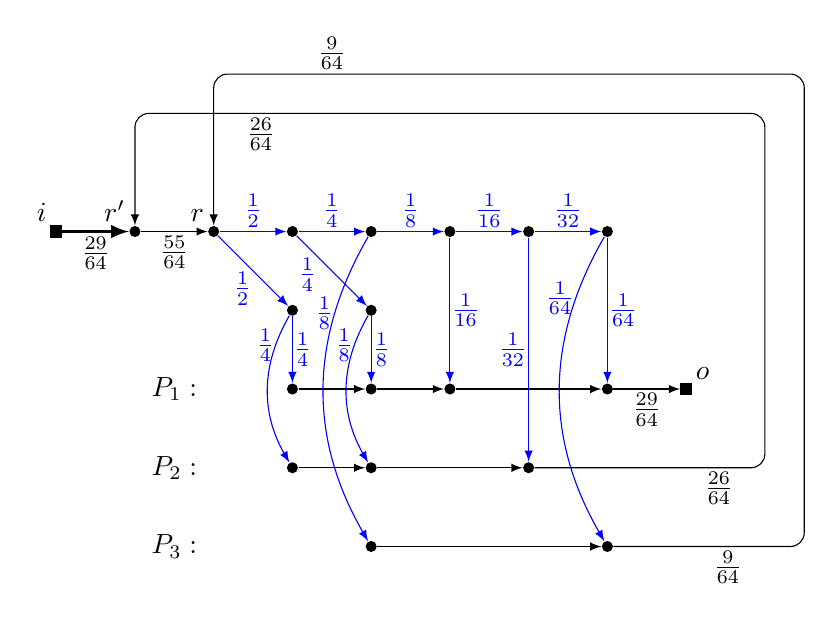
\begin{tikzpicture}[x=1cm,y=1cm,>=latex]
  \foreach \x in {0,1,...,5} {
    \node[splitter] (u\x) at (\x,4) {};
  }
  \foreach \x in {1,2} {
    \node[splitter] (v\x) at (\x,3) {};
  }
  \foreach \x in {1,2,3,5} {
    \node[splitter] (w\x) at (\x,2) {};
  }
  \foreach \x in {1,2,4} {
    \node[splitter] (y\x) at (\x,1) {};
  }
  \foreach \x in {2,5} {
    \node[splitter] (z\x) at (\x,0) {};
  }
  \node[term] (i) at (-2,4) {};
  \node[splitter] (mix) at (-1,4) {};
  \node[term] (out) at (6,2) {};
  \foreach \i/\j/\p/\q in {0/1/1/2,1/2/1/4,2/3/1/8,3/4/1/16,4/5/1/32} {
    \draw[->,fluid,blue] (u\i) -- (u\j) node[midway,above=-2pt] {$\frac{\p}{\q}$};
  }
  \foreach \l/\i/\j in {w/1/2,w/2/3,w/3/5,y/1/2,y/2/4,z/2/5} {
    \draw[->,fluid] (\l\i) -- (\l\j);
  }
  \draw[->,fluid,blue] (u0) -- (v1) node[midway,below left=-3pt] {$\frac{1}{2}$};
  \draw[->,fluid,blue] (u1) -- (v2) node[pos=0.3,below left=-3pt] {$\frac{1}{4}$};
  \draw[->,fluid,blue] (u3) -- (w3) node[midway,right=-3pt] {$\frac{1}{16}$};
  \draw[->,fluid,blue] (u4) -- (y4) node[midway,left=-3pt] {$\frac{1}{32}$};
  \draw[->,fluid,blue] (u5) -- (w5) node[midway,right=-3pt] {$\frac{1}{64}$};
  \draw[->,fluid,blue] (v1) -- (w1) node[midway,right=-3pt] {$\frac{1}{4}$};
  \draw[->,fluid,blue] (v2) -- (w2) node[midway,right=-3pt] {$\frac{1}{8}$};
  \draw[->,fluid,blue] (v1) to[bend right] node[pos=0.2,left=-3pt] {$\frac{1}{4}$} (y1);
  \draw[->,fluid,blue] (v2) to[bend right] node[pos=0.2,left=-3pt] {$\frac{1}{8}$} (y2);
  \draw[->,fluid,blue] (u2) to[bend right] node[pos=0.25,left=-3pt] {$\frac{1}{8}$}  (z2);
  \draw[->,fluid,blue] (u5) to[bend right] node[pos=0.2,left=-3pt] {$\frac{1}{64}$} (z5);
  \draw[->,saturated] (i) -- (mix) node[midway,below=-2pt] {$\frac{29}{64}$};
  \draw[->,fluid] (mix) -- (u0) node[midway,below=-2pt] {$\frac{55}{64}$};
  \draw[->,fluid] (w5) -- (out) node[midway,below=-2pt] {$\frac{29}{64}$};
  \draw[->,fluid,rounded corners=5pt] (y4) -- (7,1) node[pos=0.8,below=-2pt] {$\frac{26}{64}$}
    -- (7,5.5) -- (-1,5.5) node[pos=0.8,below=-2pt] {$\frac{26}{64}$} -- (mix);
  \draw[->,fluid,rounded corners=5pt] (z5) -- (7.5,0) node[pos=0.6,below=-2pt] {$\frac{9}{64}$}
    -- (7.5,6) -- (0,6) node[pos=0.8,above=-2pt] {$\frac{9}{64}$} -- (u0);
  \node (u) at (-0.5,2) {$P_1:$};
  \node (v) at (-0.5,1) {$P_2:$};
  \node (w) at (-0.5,0) {$P_3:$};
  \path (i) node[anchor=south east] {$i$};
  \path (mix) node[anchor=south east] {$r'$};
  \path (u0) node[anchor=south east] {$r$};
  \path (out) node[anchor=south west] {$o$};

\end{tikzpicture}

\end{document}